% The 8th Joint Workshop on Machine Perception and Robotics
% --MPR 2012 Fukaoka, Japan, Oct. 16-17, 2012

% This file is edited based on the formatting of IEEE Conference Proceedings

% Edit it to your own paper. You can modify this file and MPR-head.tex
%% This file contains instructions on preparing your own paper for IEEE conference
%% but you can also use it as a LaTeX template for your own paper.
%% Some of the settings (mainly margins) are changed.
%% only A4 paper is allowed, 10pt normal size text and we use conference
%% option of the IEEEtran style file.
%% IEEEtran.cls (at least 2005/09/13 version V1.6c) can be downloaded from IEEE
%% Make sure that it is located in a path that LaTeX can find it.
%% The pdf file is produced by using pdflatex command.
%% If you want to use dvi -> ps -> pdf then you will need
%% to add/change the packages and use eps figures.
%%
\documentclass[conference,10pt,a4paper]{IEEEtran}
%\usepackage[pdftex]{graphicx}
\usepackage{graphicx}
\usepackage{diagbox}
\usepackage[colorlinks,linkcolor=blue]{hyperref}

\addtolength {\topmargin}{-1truemm}
\textwidth 184truemm
\textheight 235truemm
\columnsep 4truemm
%
\evensidemargin -11truemm
\oddsidemargin -11truemm

%% bare_conf.tex 
%% V1.2
%% 2002/11/18
%% by Michael Shell
%% mshell@ece.gatech.edu
%% 
%% NOTE: This text file uses MS Windows line feed conventions. When (human)
%% reading this file on other platforms, you may have to use a text
%% editor that can handle lines terminated by the MS Windows line feed
%% characters (0x0D 0x0A).
%% 
%% This is a skeleton file demonstrating the use of IEEEtran.cls 
%% (requires IEEEtran.cls version 1.6b or later) with an IEEE conference paper.
%% 
%% Support sites:
%% http://www.ieee.org
%% and/or
%% http://www.ctan.org/tex-archive/macros/latex/contrib/supported/IEEEtran/ 
%%
%% This code is offered as-is - no warranty - user assumes all risk.
%% Free to use, distribute and modify.

% *** Authors should verify (and, if needed, correct) their LaTeX system  ***
% *** with the testflow diagnostic prior to trusting their LaTeX platform ***
% *** with production work. IEEE's font choices can trigger bugs that do  ***
% *** not appear when using other class files.                            ***
% Testflow can be obtained at:
% http://www.ctan.org/tex-archive/macros/latex/contrib/supported/IEEEtran/testflow


% Also note that the "draftcls" or "draftclsnofoot", not "draft", option
% should be used if it is desired that the figures are to be displayed in
% draft mode.


% some very useful LaTeX packages include:

%\usepackage{cite}      % Written by Donald Arseneau
                        % V1.6 and later of IEEEtran pre-defines the format
                        % of the cite.sty package \cite{} output to follow
                        % that of IEEE. Loading the cite package will
                        % result in citation numbers being automatically
                        % sorted and properly "ranged". i.e.,
                        % [1], [9], [2], [7], [5], [6]
                        % (without using cite.sty)
                        % will become:
                        % [1], [2], [5]--[7], [9] (using cite.sty)
                        % cite.sty's \cite will automatically add leading
                        % space, if needed. Use cite.sty's noadjust option
                        % (cite.sty V3.8 and later) if you want to turn this
                        % off. cite.sty is already installed on most LaTeX
                        % systems. The latest version can be obtained at:
                        % http://www.ctan.org/tex-archive/macros/latex/contrib/supported/cite/

%\usepackage{graphicx}  % Written by David Carlisle and Sebastian Rahtz
                        % Required if you want graphics, photos, etc.
                        % graphicx.sty is already installed on most LaTeX
                        % systems. The latest version and documentation can
                        % be obtained at:
                        % http://www.ctan.org/tex-archive/macros/latex/required/graphics/
                        % Another good source of documentation is "Using
                        % Imported Graphics in LaTeX2e" by Keith Reckdahl
                        % which can be found as esplatex.ps and epslatex.pdf
                        % at: http://www.ctan.org/tex-archive/info/

% However, be warned that pdflatex will require graphics to be in PDF
% (not EPS) format and will preclude the use of PostScript based LaTeX
% packages such as psfrag.sty and pstricks.sty. IEEE conferences typically
% allow PDF graphics (and hence pdfLaTeX). However, IEEE journals do not
% (yet) allow image formats other than EPS or TIFF. Therefore, authors of
% journal papers should use traditional LaTeX with EPS graphics.
%
% The path(s) to the graphics files can also be declared: e.g.,
%\graphicspath{{../figures/}}
% if the graphics files are not located in the same directory as the
% .tex file. This can be done in each branch of the conditional above
% (after graphicx is loaded) to handle the EPS and PDF cases separately.
% In this way, full path information will not have to be specified in
% each \includegraphics command.
%
% Note that, when switching from latex to pdflatex and vice-versa, the new
% compiler will have to be run twice to clear some warnings.


%\usepackage{psfrag}    % Written by Craig Barratt, Michael C. Grant,
                        % and David Carlisle
                        % This package allows you to substitute LaTeX
                        % commands for text in imported EPS graphic files.
                        % In this way, LaTeX symbols can be placed into
                        % graphics that have been generated by other
                        % applications. You must use latex->dvips->ps2pdf
                        % workflow (not direct pdf output from pdflatex) if
                        % you wish to use this capability because it works
                        % via some PostScript tricks. Alternatively, the
                        % graphics could be processed as separate files via
                        % psfrag and dvips, then converted to PDF for
                        % inclusion in the main file which uses pdflatex.
                        % Docs are in "The PSfrag System" by Michael C. Grant
                        % and David Carlisle. There is also some information 
                        % about using psfrag in "Using Imported Graphics in
                        % LaTeX2e" by Keith Reckdahl which documents the
                        % graphicx package (see above). The psfrag package
                        % and documentation can be obtained at:
                        % http://www.ctan.org/tex-archive/macros/latex/contrib/supported/psfrag/

\usepackage{subfigure} % Written by Steven Douglas Cochran
                        % This package makes it easy to put subfigures
                        % in your figures. i.e., "figure 1a and 1b"
                        % Docs are in "Using Imported Graphics in LaTeX2e"
                        % by Keith Reckdahl which also documents the graphicx
                        % package (see above). subfigure.sty is already
                        % installed on most LaTeX systems. The latest version
                        % and documentation can be obtained at:
                        % http://www.ctan.org/tex-archive/macros/latex/contrib/supported/subfigure/

\usepackage{url}       % Written by Donald Arseneau
                        % Provides better support for handling and breaking
                        % URLs. url.sty is already installed on most LaTeX
                        % systems. The latest version can be obtained at:
                        % http://www.ctan.org/tex-archive/macros/latex/contrib/other/misc/
                        % Read the url.sty source comments for usage information.

%\usepackage{stfloats}  % Written by Sigitas Tolusis
                        % Gives LaTeX2e the ability to do double column
                        % floats at the bottom of the page as well as the top.
                        % (e.g., "\begin{figure*}[!b]" is not normally
                        % possible in LaTeX2e). This is an invasive package
                        % which rewrites many portions of the LaTeX2e output
                        % routines. It may not work with other packages that
                        % modify the LaTeX2e output routine and/or with other
                        % versions of LaTeX. The latest version and
                        % documentation can be obtained at:
                        % http://www.ctan.org/tex-archive/macros/latex/contrib/supported/sttools/
                        % Documentation is contained in the stfloats.sty
                        % comments as well as in the presfull.pdf file.
                        % Do not use the stfloats baselinefloat ability as
                        % IEEE does not allow \baselineskip to stretch.
                        % Authors submitting work to the IEEE should note
                        % that IEEE rarely uses double column equations and
                        % that authors should try to avoid such use.
                        % Do not be tempted to use the cuted.sty or
                        % midfloat.sty package (by the same author) as IEEE
                        % does not format its papers in such ways.

\usepackage{amsmath}   % From the American Mathematical Society
                        % A popular package that provides many helpful commands
                        % for dealing with mathematics. Note that the AMSmath
                        % package sets \interdisplaylinepenalty to 10000 thus
                        % preventing page breaks from occurring within multiline
                        % equations. Use:
\interdisplaylinepenalty=2500
                        % after loading amsmath to restore such page breaks
                        % as IEEEtran.cls normally does. amsmath.sty is already
                        % installed on most LaTeX systems. The latest version
                        % and documentation can be obtained at:
                        % http://www.ctan.org/tex-archive/macros/latex/required/amslatex/math/



% Other popular packages for formatting tables and equations include:

\usepackage{array}
% Frank Mittelbach's and David Carlisle's array.sty which improves the
% LaTeX2e array and tabular environments to provide better appearances and
% additional user controls. array.sty is already installed on most systems.
% The latest version and documentation can be obtained at:
% http://www.ctan.org/tex-archive/macros/latex/required/tools/

% Mark Wooding's extremely powerful MDW tools, especially mdwmath.sty and
% mdwtab.sty which are used to format equations and tables, respectively.
% The MDWtools set is already installed on most LaTeX systems. The lastest
% version and documentation is available at:
% http://www.ctan.org/tex-archive/macros/latex/contrib/supported/mdwtools/


% V1.6 of IEEEtran contains the IEEEeqnarray family of commands that can
% be used to generate multiline equations as well as matrices, tables, etc.


% Also of notable interest:

% Scott Pakin's eqparbox package for creating (automatically sized) equal
% width boxes. Available:
% http://www.ctan.org/tex-archive/macros/latex/contrib/supported/eqparbox/



% Notes on hyperref:
% IEEEtran.cls attempts to be compliant with the hyperref package, written
% by Heiko Oberdiek and Sebastian Rahtz, which provides hyperlinks within
% a document as well as an index for PDF files (produced via pdflatex).
% However, it is a tad difficult to properly interface LaTeX classes and
% packages with this (necessarily) complex and invasive package. It is
% recommended that hyperref not be used for work that is to be submitted
% to the IEEE. Users who wish to use hyperref *must* ensure that their
% hyperref version is 6.72u or later *and* IEEEtran.cls is version 1.6b 
% or later. The latest version of hyperref can be obtained at:
%
% http://www.ctan.org/tex-archive/macros/latex/contrib/supported/hyperref/
%
% Also, be aware that cite.sty (as of version 3.9, 11/2001) and hyperref.sty
% (as of version 6.72t, 2002/07/25) do not work optimally together.
% To mediate the differences between these two packages, IEEEtran.cls, as
% of v1.6b, predefines a command that fools hyperref into thinking that
% the natbib package is being used - causing it not to modify the existing
% citation commands, and allowing cite.sty to operate as normal. However,
% as a result, citation numbers will not be hyperlinked. Another side effect
% of this approach is that the natbib.sty package will not properly load
% under IEEEtran.cls. However, current versions of natbib are not capable
% of compressing and sorting citation numbers in IEEE's style - so this
% should not be an issue. If, for some strange reason, the user wants to
% load natbib.sty under IEEEtran.cls, the following code must be placed
% before natbib.sty can be loaded:
%
% \makeatletter
% \let\NAT@parse\undefined
% \makeatother
%
% Hyperref should be loaded differently depending on whether pdflatex
% or traditional latex is being used:
%
%\ifx\pdfoutput\undefined
%\usepackage[hypertex]{hyperref}
%\else
%\usepackage[pdftex,hypertexnames=false]{hyperref}
%\fi
%
% Pdflatex produces superior hyperref results and is the recommended
% compiler for such use.



% *** Do not adjust lengths that control margins, column widths, etc. ***
% *** Do not use packages that alter fonts (such as pslatex).         ***
% There should be no need to do such things with IEEEtran.cls V1.6 and later.


% correct bad hyphenation here
\hyphenation{op-tical net-works semi-conduc-tor IEEEtran}



\begin{document}

% paper title
\title{Semantic Segmentation of 3D LiDAR Data at Dynamic Urban Scenes}


% avoiding spaces at the end of the author lines is not a problem with
% conference papers because we don't use \thanks or \IEEEmembership


\author{\authorblockN
	{Biao Gao\authorrefmark{1},
		Jilin Mei\authorrefmark{1}, 
		Donghao Xu\authorrefmark{1},
		Xijun Zhao\authorrefmark{2},
		Wen Yao\authorrefmark{2},
		Huijing Zhao\authorrefmark{1}}
\authorblockA{\authorrefmark{1}Peking University, Beijing, China}
\authorblockA{\authorrefmark{2}China North Vehicle Research Institute, Beijing, China}}


% use only for invited papers
%\specialpapernotice{(Invited Paper)}

% make the title area
\maketitle

\begin{abstract}
This work studies semantic segmentation of 3D LiDAR data at dynamic urban scenes. LiDAR data plays an important role of perception in autonomous driving system. However, most semantic segmentation methods and datasets are designed for camera data nowadays. In this work, we propose a method which can generate semantic segmentation of LiDAR data and we evaluate its performance on a new 3D point cloud dataset collected in dynamic urban scenes by our driving platform. The experiments show that our method can recognize more kinds of labels and achieve an impressive result in dynamic urban scenes.
\end{abstract}

% no key words

\section{Introduction}
% no \PARstart
	Scene understanding is crucial for the safe and efficient navigation of autonomous vehicles in complex and dynamic environments, and semantic segmentation is a key technique. 3D LiDAR has been used as one of the main sensors in many prototyping systems for fully autonomous driving\cite{urmson2008autonomous}. Semantic segmentation using 3D LiDAR data is illustrated in Fig. \ref{fig:dynamiccampus}, where given a frame of input data (a), the problem is to find a meaningful label (i.e., object class in this research) for each pixel, super-pixel or region of the data (b). As 3D LiDAR is a 2.5D sensing of the surroundings, it can be represented equivalently in the form of a range image (c)-(d) in the polar coordinate system, and the problem of semantic segmentation can be solved by using either 3D points or range images as the input.
	
	Semantic segmentation using 3D LiDAR data from outdoor scenes has been studied since the past decade \cite{urmson2008autonomous,moosmann2009segmentation,douillard2011segmentation}. The traditional process in these works \cite{munoz2009onboard,zhao2010scene} includes the following steps: (1) preprocessing to divide a whole dataset into locally consistent small units, such as voxels, segments or clusters; (2) extracting a sequence of predefined features; (3) learning a classifier via SVM, random forest etc.; and (4) refining the results using a method such as conditional random field by considering the spatial consistency among neighboring units. On one hand, the criteria of units in preprocessing are empirically defined, for example, the size of voxels\cite{hackel2017isprs}; one the other hand, the traditional methods depend on carefully designed discriminative features, and their adaptability to different scenes remains an open challenge.
	
	\begin{figure}
		\centering
		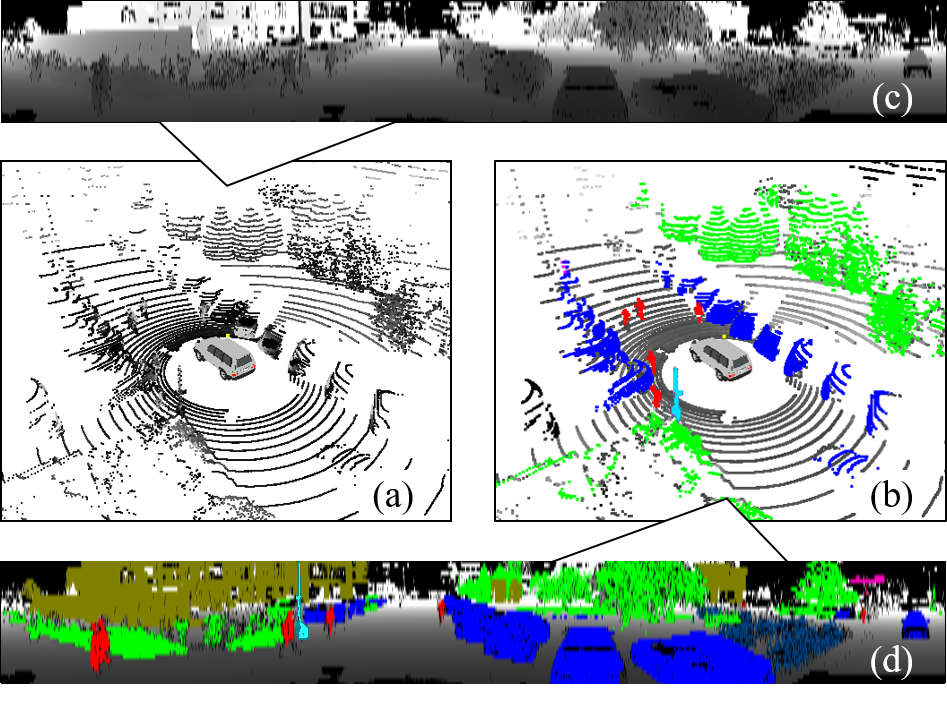
\includegraphics[width=0.5\textwidth]{fig/Fig1.png}
		\caption{The semantic segmentation for dynamic scene. (a) and (c) show the input data in two kinds of formats, i.e., the raw 3D point clouds and range frame. (b) and (d) show the semantic segmentation results.}
		\label{fig:dynamiccampus}
	\end{figure}	
	
	The recent success of deep learning in image semantic segmentation has provided new approaches\cite{garcia2017review}. These methods remove the dependence on handcrafted features in an end-to-end manner. Especially, the propose of FCN-based methods\cite{long2015fully} where the semantic segmentation is converted into a pixel-wise classification to reduce the dependence of unit's definition in preprocessing. However, these methods also have substantial demands for finely labeled data\cite{garcia2017review}, and few 3D LiDAR datasets with annotation at the point level to support autonomous driving applications are publicly available. Therefore, the attempts of a point-wise segmentation method for 3D LiDAR data and a fine annotation dataset are necessary.
	
	In this paper, we propose a new 3D LiDAR data semantic segmentation method that takes the range frame as input and make a point-wise classification via deep neural network. We evaluate its performance on a new 3D point cloud dataset collected in dynamic urban scenes by our driving platform. The experiments show that our method can recognize more kinds of labels and achieve an impressive result in dynamic urban scenes.
	
	The remainder of this paper is organized as follows. Related work is discussed in Sect. \uppercase\expandafter{\romannumeral2}. In Sect. \uppercase\expandafter{\romannumeral3}, the proposed method is presented. Then, we present the experimental results in Sect. \uppercase\expandafter{\romannumeral4} and draw conclusions in Sect. \uppercase\expandafter{\romannumeral5}.
	

\section{Related works}
	\subsection{Feature-based Methods}
	Feature-based methods belong to traditional machine learning, and the general process of these methods consists of feature selection, classifier design and graphical model description.
	
	A straightforward technique is to convert semantic segmentation into a point-wise classification that includes extracting the features on each unit, concatenating the features as a vector and determining the label via a well-trained classifier. \cite{weinmann2014semantic} presents a common pipeline from feature selection to classifier training. Due to the irregular arrangement of point clouds, the authors test 5 definitions of neighborhood to achieve the best representation. Similar research is conducted in \cite{hackel2016fast}, which demonstrates the ability to address varying densities of data. A single point cloud usually contains millions of points, so evaluating the label for each point is typically computationally expensive (on the order of minutes according to \cite{hackel2016fast}). 
	
	\cite{hu2013efficient} proposes an efficient approach where speed and accuracy are satisfied simultaneously; furthermore, the average classification time can be reduced to less than 1 s. \cite{zhao2010scene} represents the raw point cloud as a 2D range image and proposes a framework for simultaneous segmentation and classification of the range image that considers both the 2D range image and 3D raw data. Straightforward approaches assume that each data unit is independent and ignore the spatial and contextual relations between units. Consequently, they can produce good results based on distinctive features. However, when the features are not discriminative, the point-wise classification will be noisy and locally inconsistent\cite{munoz2009onboard}.
	
	The neighbor elements are taken into account to make the segmentation results spatially smooth. For this purpose, graphical models such as Markov random Field (MRF) and conditional random field (CRF) are usually exploited to encode the spatial relationships. In \cite{munoz2009contextual}, the node potentials and edge potentials are both formulated with a parametric linear model, and the functional max-margin learning is used to find the optimal weights. \cite{lu2012simplified} proposes a simplified Markov network to infer the contextual relations between points. Instead of learning all the weights for the node and edge potentials in graphical models, the node potentials are calculated from a point-wise classifier, and the edge potentials are determined by the physical distance between points. 
	
	The performance of the above methods largely depends on handcrafted features. These methods are effective in fixed or regular scenarios, but for dynamic scenes, the features are empirically designed and the performance decreases.
	
	\subsection{Deep Learning Methods}
	Deep learning, especially the convolution neural network (CNN) without handcrafted features, has shown effectual performance on 2D image segmentation\cite{garcia2017review}. However, the semantic segmentation of 3D point clouds(i.e., from LiDAR sensors) is still an open research problem\cite{engelmann2017exploring} due to the irregular, not grid-aligned properties. Therefore, recent studies project the point clouds into 2D views, and some of them attempt to directly ways, for example, volumetric/voxel representations.
	
	Inspired by the success of CNN in image segmentation, the state-of-the-art image-based algorithms can be used directly after rendering 2D views from the 3D raw data. \cite{tosteberg2017semantic} projects point clouds into virtual 2D RGB images via Katz projection. Then, a pretrained CNN is used to semantically classify the images. However, this projection removes all the points that are not visible; for example, if a car is projected, all the points behind it are removed. \cite{dewan17iros} unwraps $360^\circ$ 3D LiDAR data onto a spherical 2D plane without point loss. Spherical projection is also applied in SqueezeSeg\cite{wu2017squeezeseg}, where the CNN directly outputs the point-wise label of the transformed LiDAR data and a CRF is applied to refine the outputs. \cite{piewak2018boosting} uses cylindrical projection to create the depth and reflectivity images. In \cite{caltagirone2017fast}, the point clouds are encoded by top-view images and a simple fully convolutional neural network (FCN) is used. This method can be used in real time because only elevation and density features are extracted. In \cite{lawin2017deep}, the input point cloud is projected into multiple views, such as color, depth and surface normal images. 
	
	Another type of method models the raw data in direct ways. \cite{tchapmi2017segcloud} proposes SEGCloud, where the raw 3D point cloud is preprocessed into a voxelized point cloud with a fixed grid size. Although \cite{tchapmi2017segcloud} is simple and effective, how to set the voxel size is a problem in large-scale scenes. Thus, the scene is voxelized at five different resolutions in \cite{hackel2017isprs}, and each of the five scales is handled separately by the CNN. Rather than using a fixed grid size, \cite{riegler2017octnet} proposes OctNet, where the hybrid grid-octree data structure is applied to represent the raw 3D data, and each leaf of the octree stores a pooled feature representation. PointNet\cite{qi2017pointnet} is a unified architecture that directly takes raw point clouds as input and outputs the label of each point. The scene is divided into blocks. Then, the points in each block are passed through a series of multilayer perceptrons (MLPs) to extract the local and global features. Based on \cite{qi2017pointnet}, \cite{engelmann2017exploring} extends the method to incorporate a larger-scale spatial context, and improved results are reported in both indoor and outdoor scenarios. \cite{landrieu2017large} proposes a more elegant architecture to capture contextual relations. The first step is to partition the raw point cloud into geometrically simple shapes, called super-points. The super-points are then embedded by PointNet\cite{qi2017pointnet}.
	
	Semantic segmentation with deep learning is usually implemented in a supervised manner, which requires detailed annotations. However, obtaining point-wise annotations for 3D point clouds is labor intensive and time consuming. Furthermore, few public datasets support this level of annotation. Our method belongs the former brand where the the raw 3D point clouds is converted into 2D range frame, and FCN is applied .............

\section{Methodology}

\subsection{Data Preprocessing}
The point cloud data for LiDAR is sparse and unorganized, so it is time-consuming to find neighboring relations between different points. In order to process these unorganized point cloud data with deep convolutional neural network, we convert the point cloud data into 2D range image by cylindrical projection. After that, it will be easier to implement deep convolution neural network on the LiDAR data.

After cylindrical projection, the point cloud data will be encoded as a dense matrix with shape of $[H,W,C]$. $H$ means the number of lines for the specific LiDAR sensor (such as $H=32$ for Velodyne HDL-32E). $W$ equals to the number of points within each LiDAR scan line. $C$ is the channels' number in the range image. Here, $C$ is set to 3, which represents $[Range,Intensity,Height]$ three channels.

For each point $p_k=\langle x_k,y_k,z_k\rangle$ from the raw point cloud set $P$, the value of $Range$ in range image $R$ is defined as $r_k$:
 
\begin{equation}
r_k=\sqrt{{x_k}^2+{y_k}^2+{z_k}^2},  r_k\subset [0,255]	
\end{equation} 

Similarly, the values of $Intensity$ and $Height$ are normalized into $[0,255]$. These channels are very important properties of LiDAR data, which are enough to describe various objects in dynamic urban scenes.
 
\subsection{Problem Definition}

Let $X$ denotes the range image extracted by cylindrical projection of 3D point cloud data $S$. In this kind of projection, there is a one-to-one correspondence between a 3D point in one frame point cloud data and a pixel in the range image $X$. As a result, the semantic segmentation task of 3D point cloud data is equal with giving each pixel $x$ in the range image $X$ a label $y$. The problem of this work is formulated as learning a semantic segmentation model $f_{\theta}$ which maps each pixel $x$ to a label $y\in\{1,...,K\}$, and subsequently associate $y$ to the 3D points of $S$.

\begin{equation}
f_{\theta}: x\to y \in \{1,...,K\}
\end{equation}

The data samples are in the form of range images $X$. Given a set of supervised data samples $X_l=\{x_i, y_i\}$, where $\{x_i\}$ traverses each pixel of $X$ and $\{y_i\}$ are labels for $\{x_i\}$, annotated manually by human annotators. 
In order to learning a semantic segmentation model $f_\theta$, we need to find the best parameter set $\theta^*$ that minimize a loss function $L$ as below.

\begin{equation}
\theta^{*}=\mathop{\arg\max}_{\theta}L(X_l; \theta)
\end{equation}

\subsection{Network Architecture and Loss Function}
We use a FCN (Fully Convolutional Network) architecture for this semantic segmentation task.
Compared with common deep convolutional networks, it removes last fully connected layers, and replaces them with the in-network up-sampled or de-convolutional predictions of convolutional layers as predicted feature maps. During training procedure, it generally computes cross-entropy like losses in pixel-wise, between the predicted labels and ground truths.

Our network is trained via end-to-end guided by the designed loss function. Because the number of pixels are imbalanced between different classes and a lot of invalid or unknown-class pixels, the following multi-class weighted cross entropy loss function is designed to regular the weights between imbalanced classes.

For labeled data $X_l$, we implement some changes on the widely-used definition of cross entropy, and define loss function $L_l$ as below:

\begin{equation}
\begin{split}
&\varGamma_{i,j}=\{
	\begin{array}{lr}
	\overrightarrow{\varphi_k} ,\quad\quad if \quad [y_{i,j}\neq k \quad and\quad y_{i,j}\neq0]	\\
	\overrightarrow{0} ,\quad\quad\quad\quad\quad\quad  otherwise
	\end{array}	\\
	\\
&\textit{}L_l(X_l,Y_l;\theta)=-\frac{1}{H*W}\sum_{i=0}^{H-1}\sum_{j=0}^{W-1}\sum_{k=0}^K{\varGamma_{i,j}\omega_{k}ln(P^k_{\theta}(x_{i,j}))}
\end{split}
\end{equation}

Where $\varGamma_{i,j}$ is a one-hot vector $\varphi_k$ of label $k$, if $y_{i,j}\neq k$ and $y_{i,j}\neq0$. Label 0 means invalid or unknown pixels, including many fine fragments belong to background or hard to be annotated, so we don't want to evaluate these pixels if they are predicted as non-zero labels. $\omega_{k}$ here is used to balance the sample numbers between different labels and $P^k_{\theta}(x_{i,j})$ is the probability that pixel $x_{i,j}$ be assigned a label $k$ by our semantic segmentation model with the set of parameters $\theta$.

\section{Experiment}
\subsection{Data Set}
The performance of the proposed method is evaluated on a dynamic campus data set collected by an instrumented vehicle, which has a GPS/IMU suite and a Velodyne-HDL32, as shown in Fig. \ref{fig:collect_route}. The total route contains 1375 LiDAR frames. 880 frames for training, 220 frames for validation and 275 frames for testing.

\begin{figure}[ht]
\centering
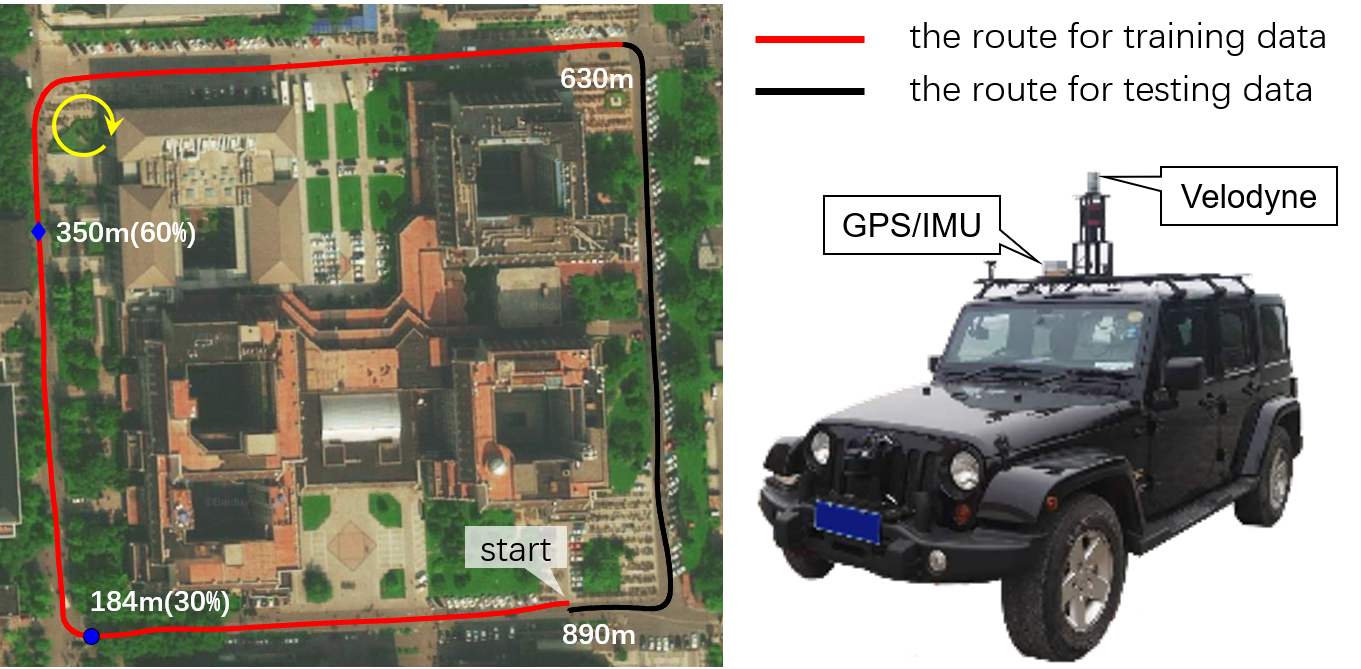
\includegraphics[width=1.0\linewidth]{fig/collect_route}
% 这个图要更新!!!!!!!!!
\caption{The routes of data collection and the platform configuration.}
\label{fig:collect_route}
\end{figure}

\begin{table*}
		\caption{Categories Distribution in Dataset}
		\label{category_distribution}
		\centering
		\small
		\renewcommand{\arraystretch}{1.5}
		\begin{tabular}{|c|c|c|c|c|c|c|c|c|}
			\hline
			 - & Pedestrian & Car & Vegetation & Sign/Pole & Building & Cyclist & Bicycle & Road	\\
			\hline
			Pixels & 458,673 & 257,239 & 4,661,880 & 80,384 & 6,579,360 & 274,991 & 1,356,518 & 16,856,614	\\
			\hline
		\end{tabular}
\end{table*}

High quality pixel-level annotation is necessary for network training. Instead of working on the raw point cloud, human annotators work on the range image where object regions are associated with the ones in adjacent frames. Annotators only need to assign the category of some region in one frame, then a series of associated regions are marked with the same label. Although sometimes the data association brings errors, it largely reduce the annotation time. 

The categories distribution in this dataset is shown in TABLE . \ref{category_distribution}. Obviously, the data distribution is imbalanced between categories. So, we apply each label an unique weight based on data distribution to reduce the influence of data imbalance.

\subsection{Setup}
Our method is implemented with a FCN (Fully Convolutional Network). The range image size is 1080x32, which width is down-sampled for efficiency. A small batch size for training sets will be better. The network is implemented with TensorFlow in the environment with NVIDIA TITAN X GPU. We use the AdamOptimizer with 1e-5 learning rate.

It's important to aware that our data frames are captured sequentially. In order to avoid data correlation between adjacent frames, shuffling them before training process is necessary.

\subsection{Results Evaluation}
We use mPA (mean pixel accuracy) for quantitative evaluation of semantic segmentation performance. Specially, when calculating the mean pixel accuracy, unknown or invalid pixels with label 0 will not be involved in. The mPA is computed as the following formula, while $\dot{Y}_k$ is the predicted pixel set with label $k$ and $Y_k$ is the ground truth pixel set.

\begin{equation}
mPA = \dfrac{1}{K}*\sum_{k=1}^{K}\dfrac{\left| \dot{Y}_k \cap Y_k \right|}{\left| \dot{Y}_k\right|}
\end{equation}

As shown in Table. \ref{performance} , we list the semantic segmentation performance (mPA) of each label, and use the result trained with original cross-entropy as baseline for comparison. Obviously, most categories achieve higher mPA performance after use our proposed method with weighted loss function. Especially, the \textit{pedestrian} label gets 37\% accuracy increase, and not only the category with fewer samples gets higher accuracy, but also the category with large amounts of samples gets higher accuracy, such as the \textit{vegetation}. However, some categories like \textit{sign/pole} still don't have ideal pixel accuracy by our method. This is most likely for too few pixel samples of these categories, so the deep learning model can't fit the data well.

The qualitative semantic segmentation results are shown in Fig.\ref{fig:result_1}. Dynamic urban scene is very vivid and contains abundant categories objects and details, which is different from simple environment on highway. As we can see in Fig.\ref{fig:result_1_a}, the weighted loss leads to better performance of labels with less samples, such as the traffic sign in Box A. Similarly, Box B,C,D in Fig.\ref{fig:result_1_b} also give some improved examples.

\begin{table*}
	\caption{semantic segmentation performance (mPA)}
	\label{performance}
	\centering
	\small
	\renewcommand{\arraystretch}{1.5}
	\begin{tabular}{|c|c|c|c|c|c|c|c|c|}
		\hline
		- & Pedestrian & Car & Vegetation & Sign/Pole & Building & Cyclist & Bicycle & Road	\\
		\hline
		Baseline Model & 0.41 & 0.71 & 0.57 & 0.36 & \textbf{0.66} & 0.49 & 0.21 & \textbf{0.99}	\\
		\hline
		Weighted-Loss Model& \textbf{0.78} & \textbf{0.93} & \textbf{0.74} & \textbf{0.40} & \textbf{0.66} & \textbf{0.56} & \textbf{0.49} & \textbf{0.99}	\\
		\hline
	\end{tabular}
\end{table*}

\begin{figure*}
	\centering
	\subfigure[Weighted loss leads to better performance of labels with less samples, such as the traffic sign in Box A.]{
		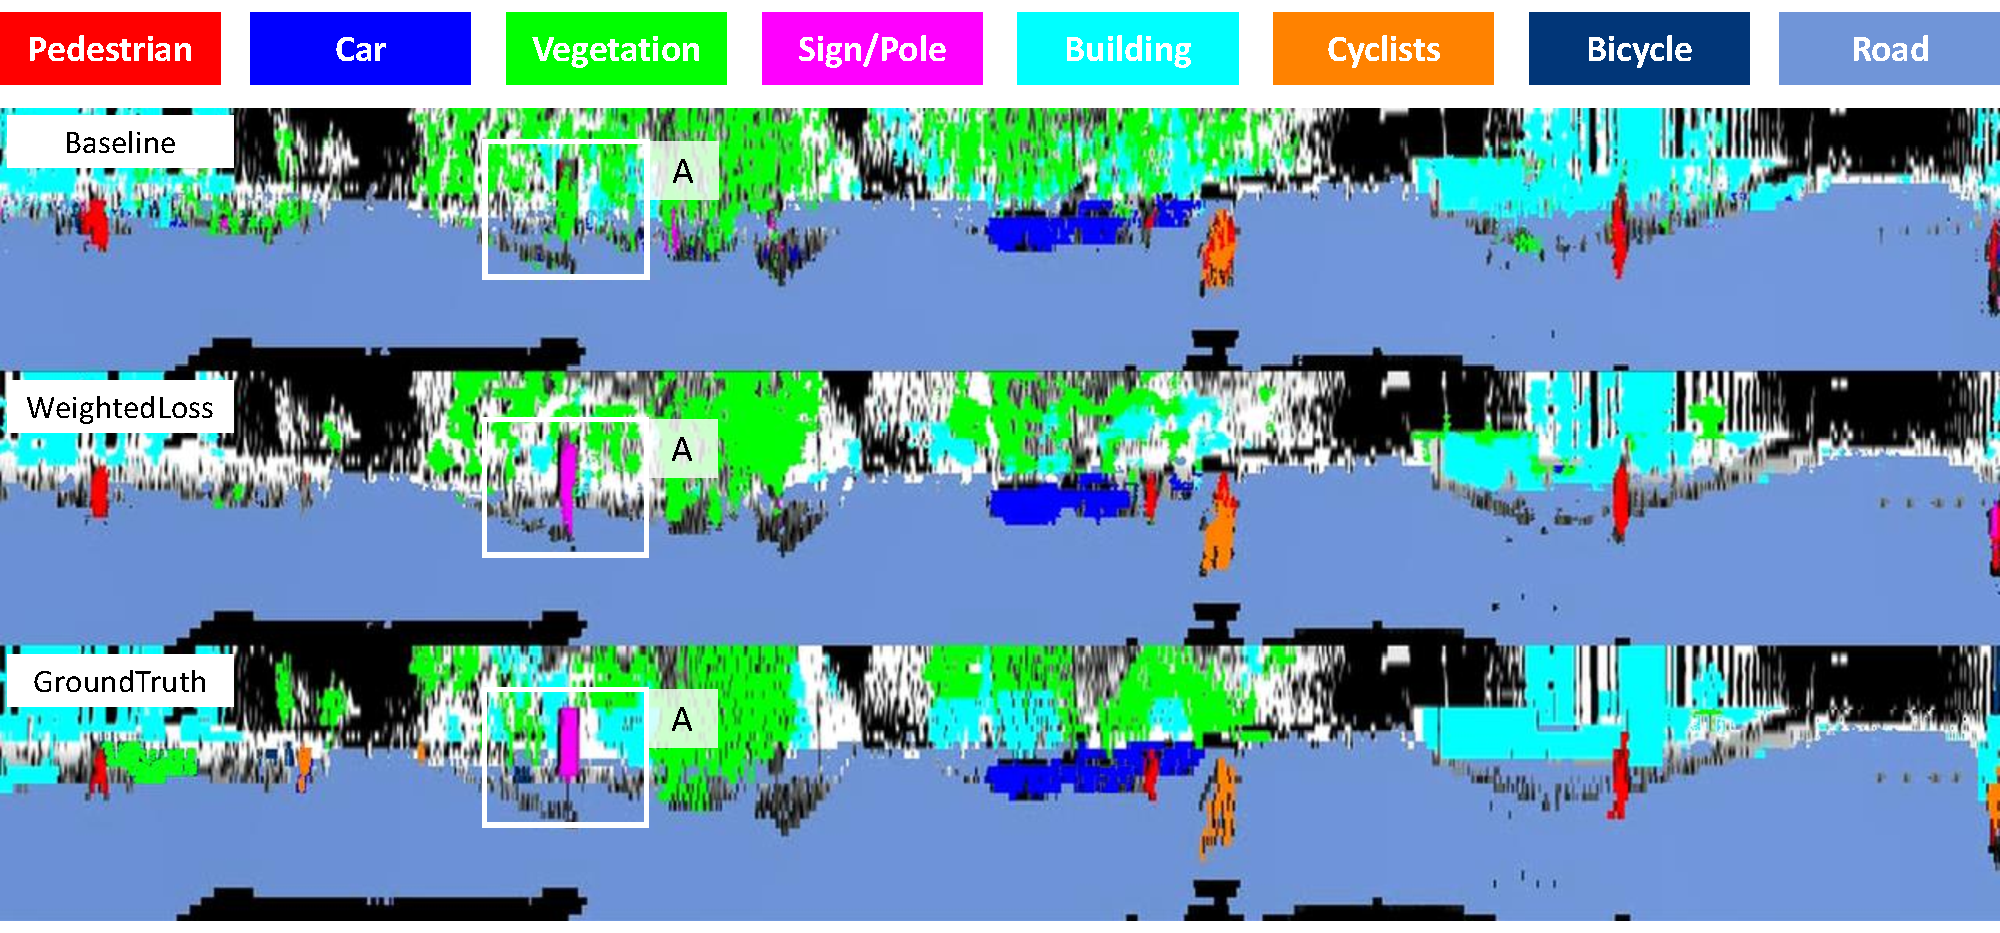
\includegraphics[width=0.9\textwidth]{fig/1.pdf}
		\label{fig:result_1_a}
	}
	\subfigure[Weighted loss version segmentation model can achieve more balanced result than the baseline. For example, Box B shows the improvement of a traffic sign's label result, and Box C,D include the results improvement of pedestrain.]{
		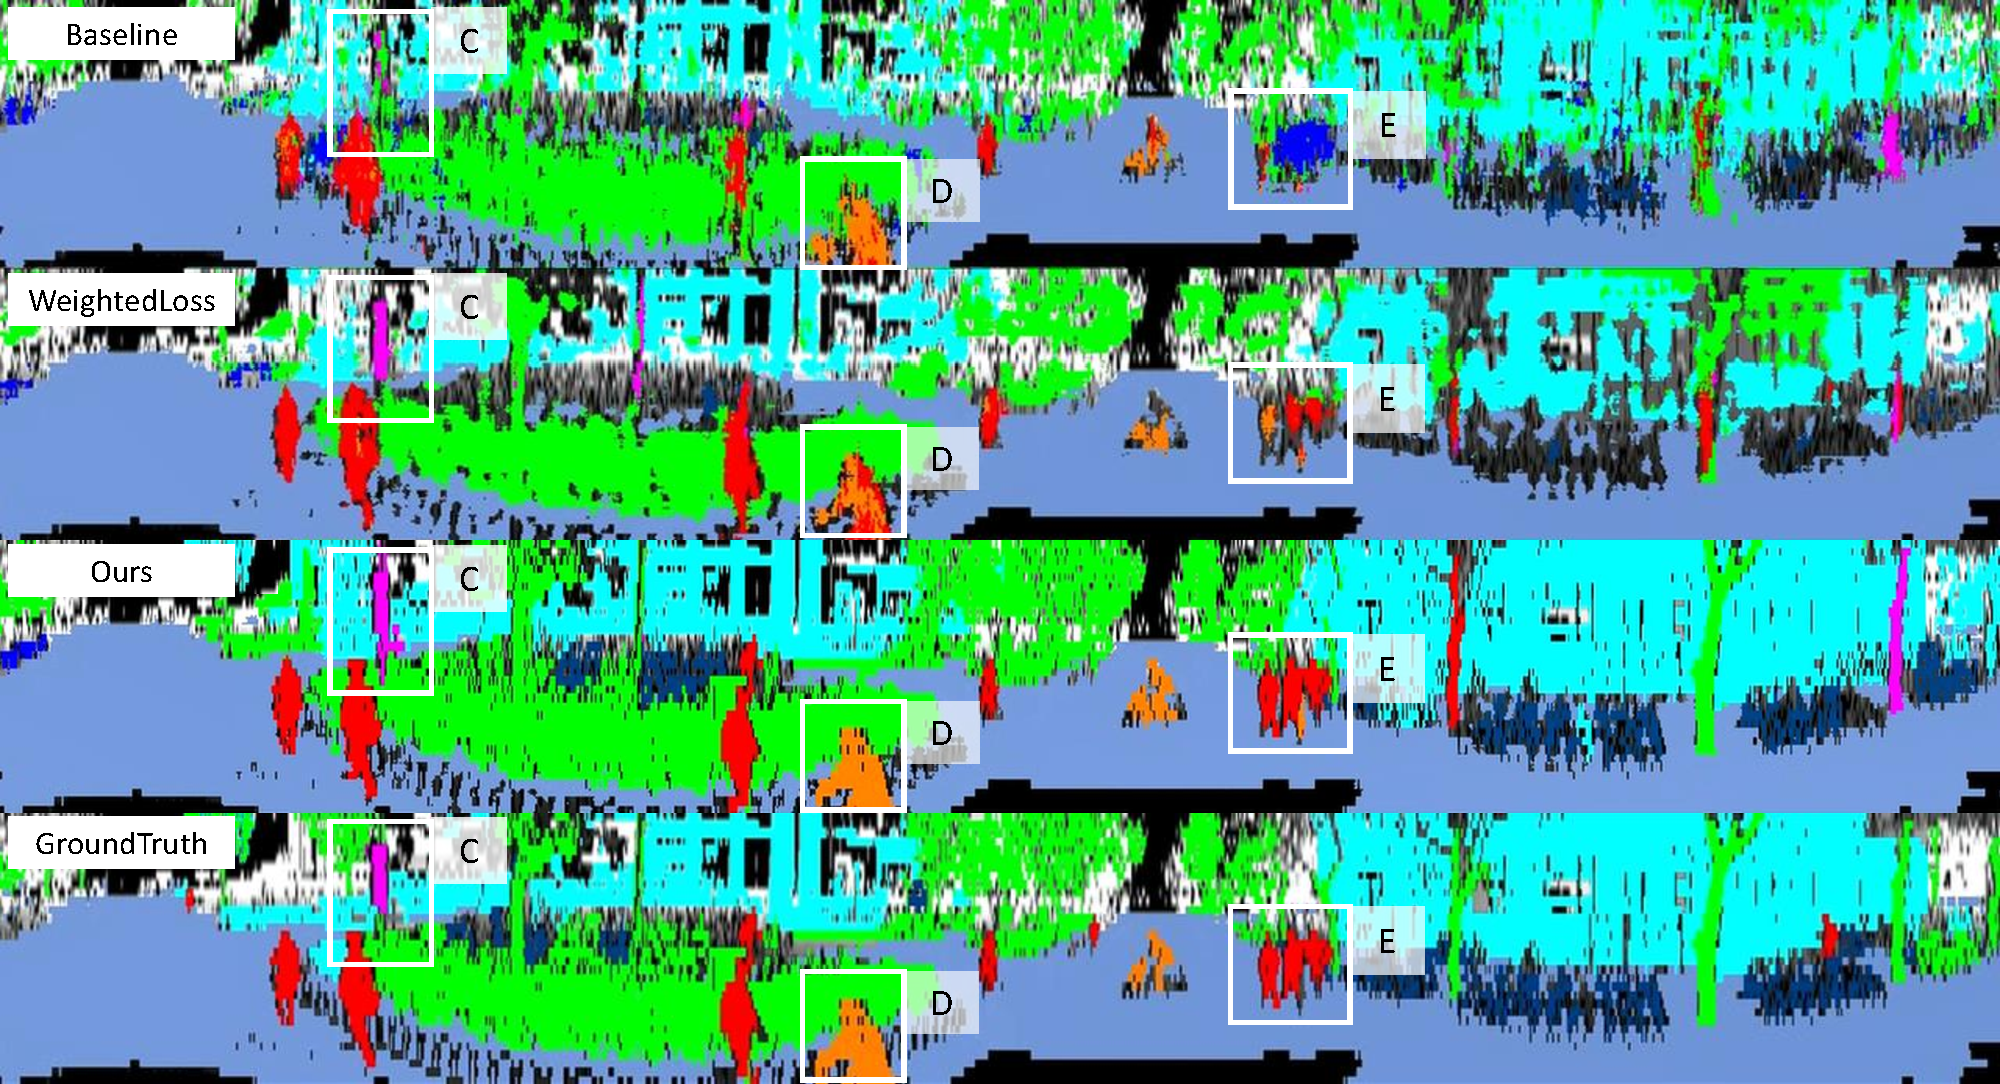
\includegraphics[width=0.9\textwidth]{fig/2.pdf}
		\label{fig:result_1_b}
	}
	\caption{Visualization result of semantic segmentation.}
	\label{fig:result_1}
\end{figure*}	

\begin{figure*} 
	\centering
	\subfigure[Confusion matrix of baseline model]{
		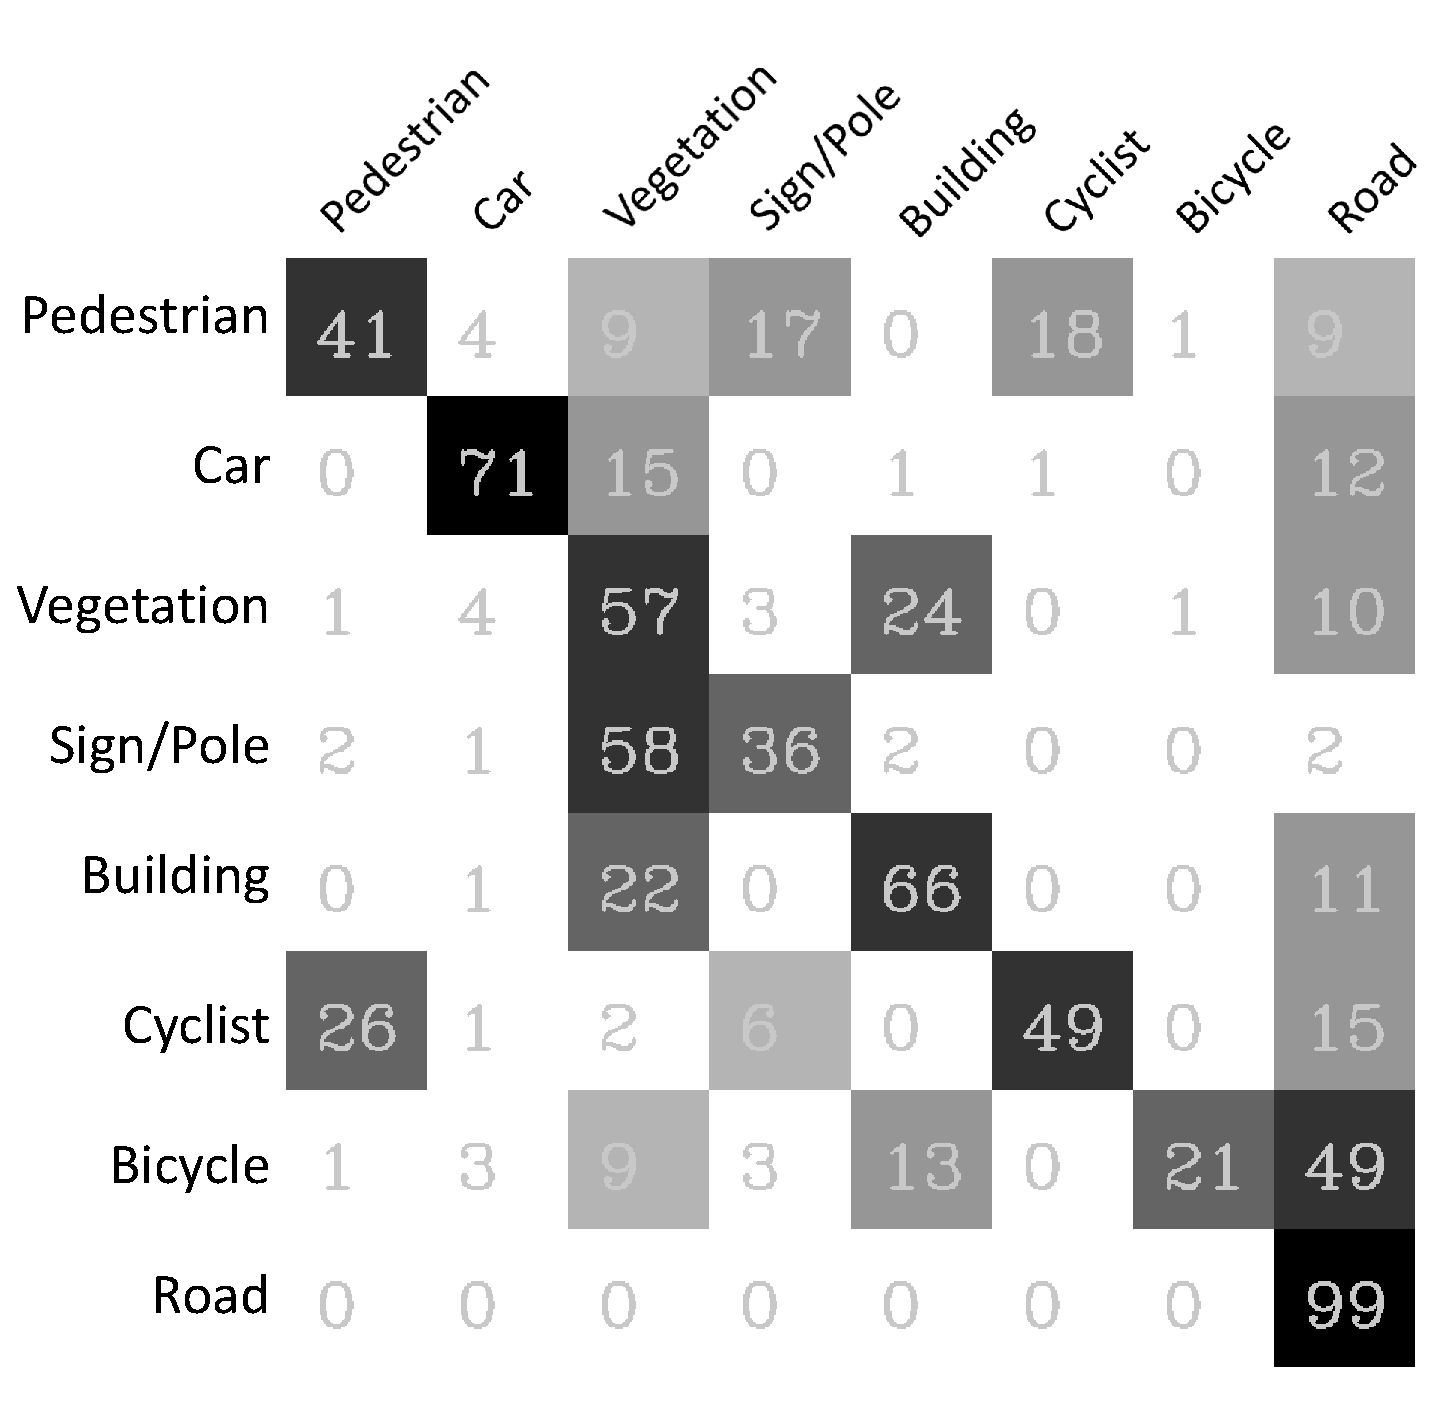
\includegraphics[width=0.35\textwidth]{fig/result_3channel_3.pdf}
		\label{fig:matrix1}
	}
	\hspace{.5in}
	\subfigure[Confustion matrix of weighted loss model]{
		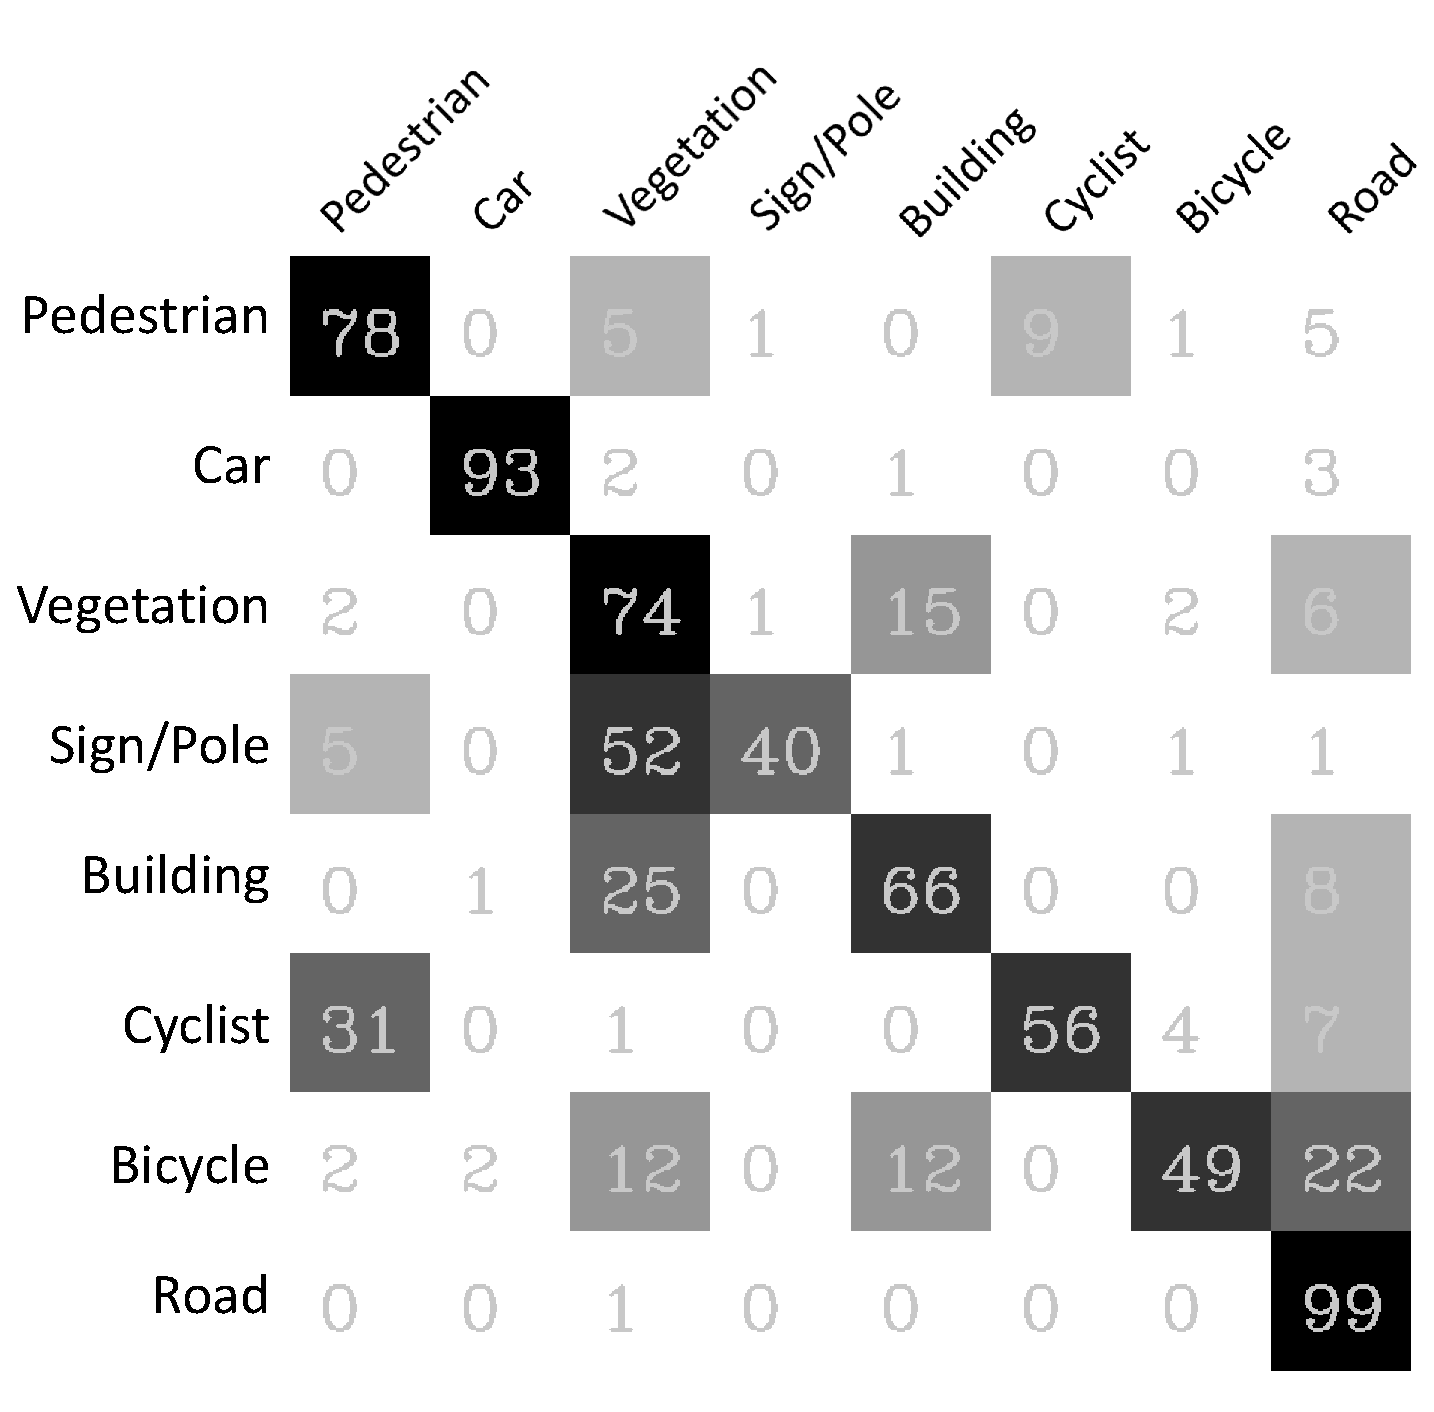
\includegraphics[width=0.35\textwidth]{fig/result_newweight_lr5.pdf}
		\label{fig:matrix2}
	}
	
	\caption{
		The confusion matrix on testing dataset, values in matrices are shown in percentage.
		\protect\\
		Rows means ground truth labels and columns means predicted labels.
	}
	\label{fig:matrix}
\end{figure*}

Fig.\ref{fig:matrix} shows the confusion matrix of baseline and weighted-loss model. It's easy to find that our model achieves a great improvement of most categories. However, some confusion between categories still exist, such as many \textit{sign/pole} samples are predicted as \textit{vegetation} and some \textit{cyclist} samples are predicted as \textit{pedestrian}. The second situation is mainly caused by the cyclists close to our vehicle, so only the upper part of the body can be seen.

By the way, there is an interesting explanation for low pixel accuracy of label \textit{sign/pole}. As shown in Fig.\ref{fig:result_1_b}, we can find that some trees trunks are labeled by \textit{sign/pole}. This is mainly because of the high reflective moth-proofing paint on the trunks, which has high value of intensity and shape as a pole, just like the traffic sign. In order to deal with this situation, maybe object-level information needs to be imported.


\section{Conclusion}
This paper proposes a semantic segmentation method of 3D LiDAR data at dynamic urban scenes. We convert the LiDAR data into the form of range images and use a fully convolutional network to predict the semantic segmentation result. We use our new dataset for evaluation, and find the weighted loss distinctly improves the pixel accuracy performance.

There are still much work need to be done in the future. In order to further improve the semantic segmentation performance, object-level information, spacial and temporal constraints between samples will be addressed on.






\begin{thebibliography}{10}

\bibitem{eason} G. Eason, B. Noble, and I. N. Sneddon, ``On certain integrals of
Lipschitz-Hankel type involving products of Bessel functions,'' {\em Phil.
Trans. Roy. Soc. London}, vol. A247, pp. 529--551, April 1955.


% use section* for acknowledgement
\section*{Acknowledgment}

The preferred spelling of the word "acknowledgment" in America is without
an "e" after the "g". Try to avoid the stilted expression, "One of us
(R.B.G.) thanks ...". Instead, try "R.B.G. thanks ...". Put sponsor
acknowledgments in the unnumbered footnote on the first page.


\bibliographystyle{IEEEtran}
\bibliography{myref}


% that's all folks
\end{document}
